%diagram
\begin{center}
\begin{figure}[h]
	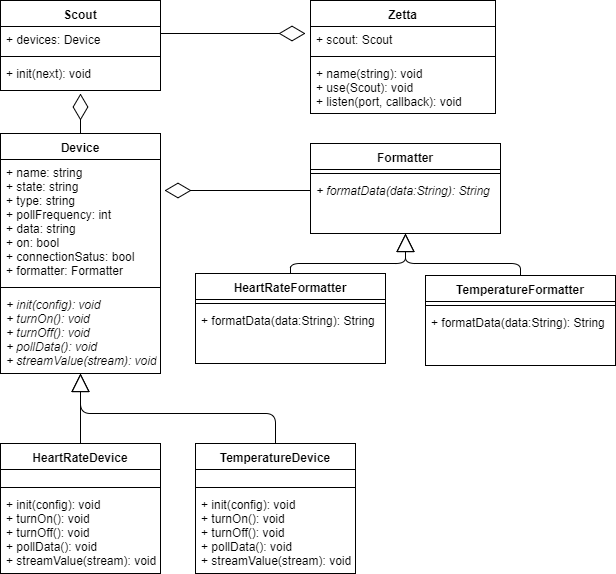
\includegraphics[width=15cm, height=13cm]{DataCollection/DataCollectionDiagram.png}
\end{figure}
\end{center}
%description
Because we used the Zetta IoT platform, we used their architecture for collecting the data from the actual devices. 
\begin{itemize}
	\item \textbf{Zetta}\\
	Zetta is the class that takes care of all the connection problems. It is a node.js server which is being used as a hub for devices. This server is then linked to another Zetta server on the cloud which exposes this API to the rest of the modules.

	\item \textbf{Scout}\\
	The Scout is responsible for finding new devices and noticing when a device is no longer connected. The Scout has a list of connected devices and relays their information back to the Zetta server.

	\item \textbf{Device}\\
	Device is another class that is provided by Zetta as an abstract interface which can facilitate functionality and monitor specific device data

	\item \textbf{HearRateDevice and TemperatureDevice}\\
	These two classes are concrete implementations of the Device class. They will be the drivers which communicate with the actual devices whether through USB, a serial connection, Bluetooth, or Wi-fi. Note also that each Device has a Formatter class.

	\item \textbf{Formatter}\\
	This class is used by the devices to format the data into specific medical or functional formats. The purpose is to pre-process the data before sending it, so as to maximise the ease of use by the other modules. It has one abstract function which would be partially or completely completed by the concrete counterparts.

	\item \textbf{HeartRateFormatter and TemperatureFormatter}\\
	These are just the concrete classes which implement the formatData() function specifically to each Device.
\end{itemize}
%design patterns
Template Method is used by the Formatter class. The formatData() function could be partially completed in the abstract class, and fully implemented in the concrete classes.

Factory Method is used in the creation of Formatters. The concrete Devices are Factories, and the the concrete Formatters are Products. Each Device must have a Formatter, but the formatter is specific for that type of device.